\documentclass{article}
\usepackage[sexy, hdr, fancy]{evan}
\setlength{\droptitle}{-4em}

\lhead{Homework 3}
\rhead{Introduction to Statistics}
\lfoot{}
\cfoot{\thepage}

\newcommand{\var}{\mathrm{Var}}
\newcommand{\cov}{\mathrm{Cov}}

\begin{document}
\title{Homework 3}
\maketitle
\thispagestyle{fancy}

\begin{enumerate}
	\item A population consists of $N$ individuals. Each individual has a certain number of friends. Suppose the count of individuals in the population with a given number of friends is as in the following table:
		\begin{center}
			\begin{tabular}{c|c}
				$k$ & number in population with $k$ friends \\
				\hline 
				0 & 1 \\
				1 & 1 \\
				$M$ & $N-4$ \\
				$2M-1$ & 1 \\
				$2M$ & 1
			\end{tabular}
		\end{center}
		where $M\ge3$ is an unknown positive integer and $N\ge7.$ A sample if size 3 is drawn without replacement and the numbers of friends for the $i$ sampled individual is denoted by $X_i,$ for $i=1, 2, 3.$

		\begin{enumerate}[(a)]
			\item Let $S$ denote the 3-tuple of elements $X_1, X_2, X_3$ that are drawn but written in increasing order. Write down a list of the 15 possible values $S$ can take on.
				\begin{soln}
					The possibilities are 
					\begin{align*}
						&(0, 1, M)\quad(0, 1, 2M-1) \quad (0, 1, 2M) \quad (0, 2M-1, 2M)\quad (1, 2M-1, 2M) \\
						&(0, M, M)\quad(1, M, M)\quad(M, M, 2M-1)\quad(M, M, 2M)\quad (M, M, M) \\
						&(0, M, 2M-1)\quad(0, M, 2M)\quad(1, M, 2M-1)\quad(1, M, 2M)\quad(M, 2M-1, 2M)
					\end{align*}
				\end{soln}

			\item Make a table giving the PMF of $S.$
				\begin{soln}
					Any event without $M$ can only happen in 1 way since there is only 1 individual of each of the number of friends 0, 1, $2M-1, 2M.$ 

					For $(0, 1, M),$ there is only 1 way to choose the individuals with 0 and 1 friends, and $N-4$ ways to choose the one with $M$ friends, so this can happen in $N-4$ ways. Similarly for $(0, M, 2M-1)$ and $(0, M, 2M)$ and $(1, M, 2M-1)$ and $(1, M, 2M)$ and $(M, 2M-1, 2M).$

					For $(0, M, M),$ there is 1 way to choose the individual with 0 friends, and $\binom{N-4}{2}$ ways to choose the 2 with $M$ friends. Similarly for $(1, M, M)$ and $(M, M, 2M-1)$ and $(M, M, 2M).$ 

					For $(M, M, M),$ there are $\binom{N-4}{3}$ ways to choose from the $N-4$ people with $M$ friends each. 

					There are $\binom{N}{3}$ ways to form groups of 3, the PMF for $S$ can be summarized as:
					\begin{center}
						\begin{tabular}{c||c|c|c|c}
							$s$ & $\begin{matrix}
								(0, 1, 2M-1) \\
								(0, 1, 2M) \\
								(0, 2M-1, 2M) \\
								(1, 2M-1, 2M)
							\end{matrix}$ & $\begin{matrix}
								(0, 1, M) \\
								(0, M, 2M-1) \\
								(0, M, 2M) \\
								(1, M, 2M-1) \\
								(1, M, 2M) \\
								(M, 2M-1, 2M)
							\end{matrix}$ & $\begin{matrix}
								(0, M, M) \\
								(1, M, M) \\
								(M, M, 2M-1) \\
								(M, M, 2M)
							\end{matrix}$ & $(M, M, M)$ \\
							\hline
							$p_S(s)$ & $1/\binom{N}{3}$ & $(N-4)/\binom{N}{3}$ & $\binom{N-4}{2}/\binom{N}{3}$ & $\binom{N-4}{3}/\binom{N}{3}$
						\end{tabular}
					\end{center}

				\end{soln}

			\item Compute the PMF of $Y=X_1+X_2+X_3.$ Note that $Y$ is a function of $S$ the set that is drawn.
				\begin{soln}
					The unique values of $Y$ along with the ways to form them are:
					\begin{align*}
						2M &\to (0, 1, 2M-1)\quad(0, M, M) \\
						2M+1 &\to (0, 1, 2M)\quad(1, M, M) \\
						4M-1 &\to (0, 2M-1, 2M)\quad(M, M, 2M-1) \\
						4M &\to (1, 2M-1, 2M)\quad(M, M, 2M) \\
						M+1 &\to (0, 1, M) \\
						3M-1 &\to (0, M, 2M-1) \\
						3M &\to (0, M, 2M)\quad(1, M, 2M-1)\quad(M, M, M) \\
						3M+1 &\to (1, M, 2M) \\
						5M-1 &\to (M, 2M-1, 2M)
					\end{align*}
					so the probability of each value of $Y$ is the sum of the probability masses of the triples that form them. Thus the PMF of $Y$ can be summarized as:

					\begin{center}
						\begin{tabular}{c||c|c|c|c|c}
							$y$ & $M+1$ & $2M$ & $2M+1$ & $3M-1$ & $3M$ \\
							\hline
							$p_Y(y)$ & $\displaystyle\frac{N-4}{\binom{N}{3}}$ & $\displaystyle\frac{1+\binom{N-4}{2}}{\binom{N}{3}}$ & $\displaystyle\frac{1+\binom{N-4}{2}}{\binom{N}{3}}$ & $\displaystyle\frac{N-4}{\binom{N}{3}}$ & $\displaystyle\frac{2(N-4)+\binom{N-4}{3}}{\binom{N}{3}}$ \\
							\hline
							$y$ & $3M+1$ & $4M-1$ & $4M$ & $5M-1$ & \\
							\hline
							 $p_Y(y)$ & $\displaystyle\frac{N-4}{\binom{N}{3}}$ & $\displaystyle\frac{1+\binom{N-4}{2}}{\binom{N}{3}}$ & $\displaystyle\frac{1+\binom{N-4}{2}}{\binom{N}{3}}$ & $\displaystyle\frac{N-4}{\binom{N}{3}}$ & 
						\end{tabular}
					\end{center}

				\end{soln}

			\item Compute the PMF of $\bar{X}=(X_1+X_2+X_3)/3$ and use this to determine $E[\bar{X}].$
				\begin{soln}
					Since $\bar{X}=Y/3,$ it has the same underlying probabilities, just the values are changed. The PMF of $\bar{X}$ can be summarized as:

					\begin{center}
						\begin{tabular}{c||c|c|c|c|c}
							$\bar{x}$ & $(M+1)/3$ & $2M/3$ & $(2M+1)/3$ & $(3M-1)/3$ & $M$ \\
							\hline
							$p_{\bar{X}}(\bar{x})$ & $\displaystyle\frac{N-4}{\binom{N}{3}}$ & $\displaystyle\frac{1+\binom{N-4}{2}}{\binom{N}{3}}$ & $\displaystyle\frac{1+\binom{N-4}{2}}{\binom{N}{3}}$ & $\displaystyle\frac{N-4}{\binom{N}{3}}$ & $\displaystyle\frac{2(N-4)+\binom{N-4}{3}}{\binom{N}{3}}$ \\
							\hline
							$\bar{x}$ & $(3M+1)/3$ & $(4M-1)/3$ & $4M/3$ & $(5M-1)/3$ & \\
							\hline
							$p_{\bar{X}}(\bar{x})$ & $\displaystyle\frac{N-4}{\binom{N}{3}}$ & $\displaystyle\frac{1+\binom{N-4}{2}}{\binom{N}{3}}$ & $\displaystyle\frac{1+\binom{N-4}{2}}{\binom{N}{3}}$ & $\displaystyle\frac{N-4}{\binom{N}{3}}$ & 
						\end{tabular}
					\end{center}
					Then
					\begin{align*}
						E[\bar{X}] &= \sum_{\bar{x}} \bar{x}\cdot p_{\bar{X}} (\bar{x}) \\
						&= \frac{1}{\binom{N}{3}} \Bigg[(N-4)\left( \frac{M+1}{3} + \frac{3M-1}{3} + \frac{3M+1}{3} + \frac{5M-1}{3} \right) \\
						&\quad+\left( 1+\binom{N-4}{2} \right)\left( \frac{2M}{3}+\frac{2M+1}{3}+\frac{4M-1}{3}+\frac{4M}{3} \right) + \left( 2(N-4)+\binom{N-4}{3} \right)M \Bigg] \\
						&= \boxed{M}
					\end{align*} after some ugly algebra.
					
				\end{soln}

			\item Compute the population variance $\sigma^2.$ Compute $\var(\bar{X}).$ 
				\begin{soln}
					The population mean is given by \[\mu=\frac{1}{M}(1(0)+1(1)+(N-4)(M)+1(2M-1)+1(2M) = M, \] so the population variance is given by
					\begin{align*}
						\sigma^2 &= \frac{1}{N}\sum_{}^{}(x_i-\mu)^2 \\
						&= \frac{1}{N}( (0-M)^2+(1-M)^2+(2M-1-M)^2+(2M-M)^2) \\
						&= \boxed{\frac{4M^2-4M+2}{N}}
					\end{align*}

					Next, for $\var(\bar{X}),$ we use the relation \[\var(\bar{X})=E[\bar{X}^2] - (E[\bar{X}])^2 = E[\bar{X}^2]-M^2.\] Then $E[\bar{X}^2]$ is calculated similarly to $E[\bar{X}],$ replacing all $\bar{x}$ with $\bar{x}^2$ in the summation, and we get \[\var(\bar{X})=\boxed{\frac{N-3}{3N(N-1)}(4M^2-4M+2).}\]

				\end{soln}

			\item If we use $\bar{X}$ to estimate $M,$ what is the mean square error $E[(\bar{X}-M)^2]?$
				\begin{soln}
					The MSE can be rewritten as \[E[\bar{X}^2-2M\bar{X}+M^2]=E[\bar{X}^2]-2M^2+M^2=E[\bar{X}^2]-M^2 = \boxed{\frac{N-3}{3N(N-3)}(4M^2-4M+2).} \]
				\end{soln}

			\item Let $T$ denote the \textit{sample median}. Compute the PMF of $T$ and determine $E[T].$
				\begin{soln}
					Looking at the possible values of $S,$ the possible values of $T$ and the ways to generate them are:
					\begin{align*}
						1 &\to (0, 1, M)\quad(0, 1, 2M-1)\quad(0, 1, 2M) \\
						M&\to (0, M, M)\quad(0, M, 2M-1)\quad(0, M, 2M)\quad(1, M, M)\quad(1, M, 2M-1) \\ &\quad(1, M, 2M)\quad(M, M, M)\quad(M, M, 2M-1)\quad(M, M, 2M) \\
						2M-1&\to (0, 2M-1, 2M)\quad (1, 2M-1, 2M)\quad(M, 2M-1, 2M)
					\end{align*}
					The probability of each of the possible sample medians occurring is the sum of the probabilities of each of the events on the RHS occurring, so the PMF can be summarized as:
					\begin{center}
						\begin{tabular}{c||c|c|c}
							$t$ & 1 & $M$ & $2M-1$ \\
							\hline
							$p_T(t)$ & $\displaystyle\frac{(N-4) + 2(1)}{\binom{N}{3}}$ & $\displaystyle\frac{\binom{N-4}{3}+4\binom{N-4}{2}+4(N-4)}{\binom{N}{3}}$ & $\displaystyle\frac{2(1)+(N-4)}{\binom{N}{3}}$
						\end{tabular}
					\end{center}

					Thus
					\begin{align*}
						E[T] &= \sum_{t}^{}t\cdot p_T(t) \\
						&= \frac{1}{\binom{N}{3}} \left[ 1\cdot(N-2)+M\cdot\left( \binom{N-4}{3}+4\binom{N-4}{2}+4(N-4) \right)+ (2M-1)\cdot (N-4) \right] \\
						&= \boxed{M}
					\end{align*} after algebra. 
					
				\end{soln}

			\item Find an expression for $\var(T)$ and simplify it.
				\begin{soln}
					We have the relation $\var(T)=E[T^2]-(E[T])^2=E[T^2]-M^2.$ Calculating $E[T^2]$ similarly to $E[T],$ and applying the Law of the Unconscious Statistician, we find that \[\var(T)=\boxed{\frac{12}{N(N-1)}(M^2-2M+1)}\]
				\end{soln}

			\item If we use $T$ to estimate $M,$ what is the mean squared error $E[(T-M)^2]?$
				\begin{soln}
					We have 
					\begin{align*}
						E[(T-M)^2]&=E[T^2-2TM+M^2]=E[T^2]-2M\cdot E[T]+E[M^2] \\
						&=E[T^2]-2M^2+M^2=E[T^2]-M^2 \\
						&= \boxed{\frac{12}{N(N-1)}(M^2-2M+1)}
					\end{align*}			
				\end{soln}

			\item Suppose we will decide which estimator of $M$ to use (sample mean or sample median) based on which has a smaller MSE. Define the \textit{efficiency} of the sample median \textit{relative} to the sample mean to be \[\text{eff}=\frac{E[(\bar{X}-M)^2}{E[(T-M)^2]}.\] Show that this expression can be written as the product of two terms, one which is linear in $N$ and the other which is a ratio of two quadratics in $M.$
				\begin{proof}
					Substituting our expressions in from the previous parts, this is
					\begin{align*}
						\text{eff} &= \frac{\frac{N-3}{3N(N-1)}(4M^2-4M+2)}{\frac{12}{N(N-1)}(M^2-2M+1)} \\
						&= \frac{N}{36} \cdot \frac{4M^2-4M+2}{M^2-2M+1}
					\end{align*} which is in the form desired.

				\end{proof}

				\newpage
			\item Describe situations (for some integers $M$ and $N$ with $M\ge3$ and $N\ge7$) when the sample mean has a smaller MSE than the sample median. If $N>12,$ show that the sample median has a smaller MSE than the sample mean no matter what $M$ is (as long as it is at least 3).
				We first show that when $N>12$ the MSE of $\bar{X}$ is always greater than MSE of $T.$ We have 
				\begin{align*}
					\frac{N-3}{3N(N-1)}(4M^2-4M+2) &> \frac{12-3}{3N(N-1)}(4M^2-4M+2) \\
					&= \frac{3}{N(N-1)}(4M^2-4M+2)\\
					&= \frac{12}{N(N-1)}\left( M^2-M+\frac{1}{2} \right)
				\end{align*} 
				Comparing $M^2-M+\frac{1}{2}$ and $M^2-2M+1,$ we find that the former is greater than the latter whenever $M>1/2,$ but since we are given $M\ge 3,$ this is true. Thus the MSE of $\bar{X}$ is always greater than that of $T$ whenever $N>12$ and $M\ge 3,$ as desired.

				That means the situations when the MSE of $\bar{X}$ is smaller than that of $T$ can only happen when $N=7, 8, \cdots, 12.$ This is equivalent to 
				\begin{align*}
					\frac{N-3}{3N(N-1)}(4M^2-4M+2) &< \frac{12}{N(N-1)}(M^2-2M+1) \\
					\frac{N-3}{3}(4M^2-4M+2) &< 12(M^2-2M+1)
				\end{align*} Tackle these by cases.

				Case 1: $N=7.$ Then
				\begin{align*}
					\frac{4}{3}(4M^2-4M+2) &< 12(M^2-2M+1) \\
					\implies M &>\frac{7+\sqrt{14}}{5} 
				\end{align*} so whenever $M\ge 3.$

				Case 2: $N=8.$ Then
				\begin{align*}
					\frac{5}{3}(4M^2-4M+2) &< 12(M^2-2M+1) \\
					\implies M &> \frac{13+\sqrt{65}}{8} 
				\end{align*} so whenever $M\ge 3.$

				Case 3: $N=9.$ Then
				\begin{align*}
					\frac{6}{3}(4M^2-4M+2) &< 12(M^2-2M+1) \\ 
					\implies M &> 2+\sqrt{2}
				\end{align*} so whenever $M\ge 4.$

				Case 4: $N=10.$ Then 
				\begin{align*}
					\frac{7}{3}(4M^2-4M+2) &< 12(M^2-2M+1) \\
					\implies M &> \frac{11+\sqrt{77}}{4}
				\end{align*} so whenever $M\ge 5.$

				Case 5: $N=11.$ Then 
				\begin{align*}
					\frac{8}{3}(4M^2-4M+2) &< 12(M^2-2M+1) \\
					\implies M &> 5+2\sqrt{5}
				\end{align*} so whenever $M\ge 10.$

				Case 6: $N=12.$ Then
				\begin{align*}
					\frac{9}{3}(4M^2-4M+2) &< 12(M^2-2M+1) \\
					\implies M &< \frac{1}{2}
				\end{align*} but since we must have $M\ge 3,$ there are no solutions in this case.

		\end{enumerate}

	\item Complete the following:
		\begin{enumerate}[(a)]
			\item Show that if $X_i$ are iid Bernoulli random variables with success probability $p$ for some $p\in(0, 1),$ then \[\frac{1}{n}\sum_{i=1}^n X_i\to p\] as $n\to\infty.$
				\begin{proof}
					By the Central Limit Theorem, the distribution of $\bar{X}$ approaches the normal distribution with $\mu=p$ and $\sigma^2=\frac{p(1-p)}{n}.$ Thus, as $n\to\infty,$ the distribution of $\bar{X}$ approaches a distribution with $\mu=p$ and $\sigma^2=0,$ so the distribution is essentially a point mass of 1 at $p.$ Thus, $\bar{X}\to p$ as $n\to\infty.$
					
				\end{proof}

			\item In R, get an approximation to the expected value of the length of the longest run in $n$ flips of a fair coin for $n=10, 20, 30, \cdots, 250.$
				\begin{answer*}
					This was completed in RStudio. 
				\end{answer*}

			\item Plot the expected value in (a) vs $n$ and try to fit a curve of the form $y=c\log n$ for some $c$ to the data.
				\begin{soln}
					The results from the previous part are plotted below, and the generated fit was $y=0.357 + 1.438\ln x,$ where $x$ was the number of flips, and $y$ was the average of the longest run.
					\begin{center}
						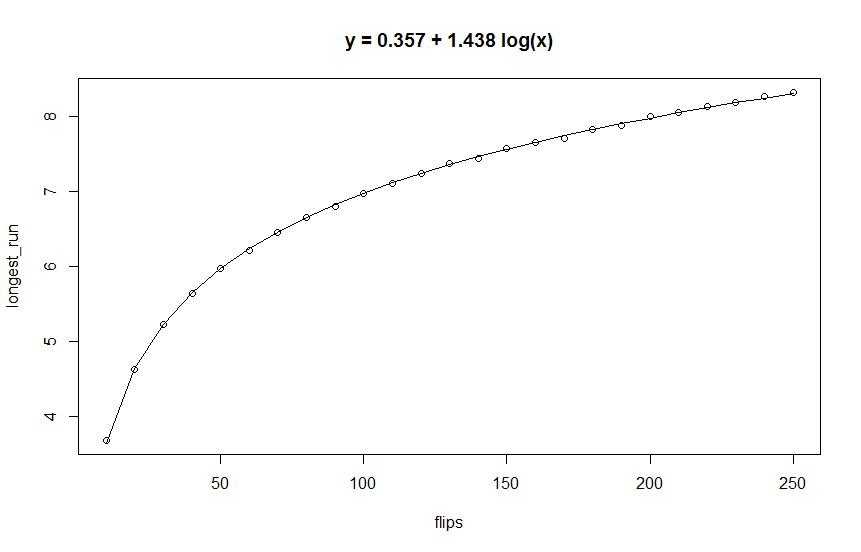
\includegraphics[width=6cm]{longest_run.png}
					\end{center}
					
				\end{soln}

			\item Use your fit in (c) to predict the expected value when $n=500.$ Then approximate the value you get using simulation and compare.
				\begin{soln}
					From the fit equation, we have \[E[R_{500}]\approx 0.357+1.438\ln500 \approx 9.2936. \] The simulation run on $n=500$ gave an expectation of 9.3033, so the two agree closely.
					
				\end{soln}
				
			\item Now, consider a Monte-Carlo approximation of the variance of a random variable. Explain why the expression \[\frac{1}{n}\sum_{i=1}^n X_i^2\] can be used to approximate $E[X^2],$ and thus why \[\frac{1}{n}\sum_{i=1}^n X_i^2 - \left( \frac{1}{n}\sum_{i=1}^n X_i \right)^2 \approx E[X^2]-\mu^2=\var(X).\]

			\item From the previous part, explain why, for large $n,$ we can approximate $\var(X)$ using the sample variance of the values $X_1, \cdots, X_n$ \[\frac{1}{n-1}\sum_{i=1}^n (X_i-\bar{X})^2.\]

			\item Take $X$ to be the length of the longest run in $n$ trials. Estimate $\var(X)$ for $n=10, 20, 30, \cdots, 250,$ and plot $\var(X)$ vs $n.$
				
		\end{enumerate}

	\item Consider sampling \textit{with replacement} using a sample of size $n$ from a population of size $N$ where each individual $i$ has two attributes $x_i, y_i.$ Let \[\sigma_{xy}=\frac{1}{N}\sum_{i=1}^N (x_i-\mu_x)(y_i-\mu_y)\] denote the population covariance between $x$ and $y$ where $\mu_x$ and $\mu_y$ denote the population means. Let $(X_i, Y_i), \, i=1, \cdots, n$ denote the $(x, y)$ values for the individuals sampled. 

		Show that the sample covariance \[s_{xy}=\frac{1}{n-1}\sum_{i=1}^n (X_i-\bar{X})(Y_i-\bar{Y})\] is unbiased for $\sigma_{xy}.$
		\begin{proof}
			We have
			\begin{align*}
				\frac{1}{n-1}\sum_{i=1}^{n} (X_i-\bar{X})(Y_i-\bar{Y}) &= \frac{1}{n-1}\sum_{i=1}^{n} (X_iY_i-X_i\bar{Y}-\bar{X}Y_i+\bar{X}\bar{Y}) \\
				&= \frac{1}{n-1}\left(\sum_{i=1}^{n} X_iY_i - \sum_{i=1}^{n} X_i \bar{Y} - \sum_{i=1}^{n} Y_i\bar{X} + \sum_{i=1}^{n} \bar{X}\bar{Y} \right) \\
				&= \frac{1}{n-1}\left( \sum_{i=1}^{n} X_iY_i - \bar{Y}\sum_{i=1}^{n} X_i - \bar{X}\sum_{i=1}^{n} Y_i + n\bar{X}\bar{Y} \right) \\
				&= \frac{1}{n-1}\left( \sum_{i=1}^{n} X_iY_i - n\bar{Y}\bar{X}-n\bar{X}\bar{Y}+n\bar{X}\bar{Y} \right) \\
				&= \frac{1}{n-1}\left( \sum_{i=1}^{n} X_iY_i - n\bar{X}\bar{Y} \right)
			\end{align*} 
			Then taking the expectation of this, we have 
			\begin{align*}
				E[s_{xy}] &= E\left[ \frac{1}{n-1}\left( \sum_{i=1}^{n} X_iY_i - n\bar{X}\bar{Y} \right) \right] \\
				&= \frac{1}{n-1} \left(\sum_{i=1}^{n} E[X_iY_i]-nE[\bar{X}\bar{Y}]\right) \\
			\end{align*}
			We know that $E[X_iY_i]-E[X_i]E[Y_i]=\cov(X_i, Y_i)=\sigma_{xy},$ and $E[X_i]=\mu_x$ and similarly for $Y_i,$ so then \[E[X_iY_i]=\sigma_{xy}+\mu_x\mu_y.\] 

			Similarly, we have 
			\begin{align*}
				E[\bar{X}\bar{Y}]-E[\bar{X}]E[\bar{Y}]&=\cov(\bar{X}, \bar{Y}) \\
				&= \cov\left( \frac{1}{n}\sum_{i=1}^{n} X_i, \frac{1}{n}\sum_{i=1}^{n}Y_i \right) \\
				&= \frac{1}{n^2} \sum_{i=1}^{n}\sum_{j=1}^{n}\cov(X_i, Y_j)
			\end{align*}
			Since samples are taken with replacement, $\cov(X_i, Y_j)=0$ whenever $i\neq j,$ so in fact this sum is just \[\frac{1}{n^2}\sum_{k=1}^{n}\cov(X_k, Y_k) = \frac{1}{n^2}n\sigma_{xy} = \frac{\sigma_{xy}}{n}\] Thus \[E[\bar{X}\bar{Y}]=\frac{\sigma_{xy}}{n}+\mu_x\mu_y.\] Substituting these back into the expression for the expectation of $s_{xy},$ we have 
			\begin{align*}
				E[s_{xy}] &= \frac{1}{n-1}\left( \sum_{i=1}^{n} (\sigma_{xy}+\mu_x\mu_y) - n\left( \frac{\sigma_{xy}}{n}+\mu_x\mu_y \right) \right) \\
				&= \frac{1}{n-1} \left( n\sigma_{xy}+n\mu_x\mu_y-\sigma_{xy}-n\mu_x\mu_y \right) \\
				&= \frac{1}{n-1}(n\sigma_{xy}-\sigma_{xy}) \\
				&= \sigma_{xy}
			\end{align*} as desired.
		\end{proof}

\end{enumerate}

\section*{Chapter 7: Survey Sampling}
\begin{itemize}
	\item[45.] In the population of hospitals, the correlation of the number of beds and the number of discharges is $\rho=0.91.$ To see how $\var(\bar{Y}_R)$ would be different if the correlation were different, plot $\var(\bar{Y}_R)$ for $n=64$ as a function of $\rho$ for $-1<\rho<1.$

	\item[46.] Use the central limit theorem to sketch the approximate sampling distribution of $\bar{Y}$ for $n=64$ for the population of hospitals. Compare to the approximate sampling distribution of $\bar{Y}.$

	\item[48.] A simple random sample of 100 households located in a city recorded the number of people living in the household, $X,$ and the weekly expenditure for food, $Y.$ it is known that there are 100000 households in the city. In the sample, 
		\begin{align*}
			\sum X_i &= 320 \\
			\sum Y_i &= 10000 \\
			\sum X_i^2 &= 1250 \\
			\sum Y_i^2 &= 1100000 \\
			\sum X_iY_i &= 36000
		\end{align*}
		Neglect the finite population correction in answering the following.

		\begin{enumerate}[a.]
			\item Estimate the ratio $r=\mu_y/\mu_x.$
				\begin{soln}
					We have $\bar{X}=3.20$ and $\bar{Y}=100$ by dividing the sums by 100. 
					
					Let $R=\bar{Y}/\bar{X}$ be an estimator for $r,$ then $R=100/3.20=\boxed{31.25}$ is an estimate for $r.$

				\end{soln}

			\item Form an approximate 95\% confidence interval for $\mu_y/\mu_x.$ 
				\begin{soln}
					We need to calculate $\var(R),$ which by Theorem A is given by
					\begin{align*}
						\var(R) &\approx \frac{1}{n\mu_x^2}(r^2\sigma_x^2 + \sigma_y^2-2r\sigma_{xy}) \\
						&\approx \frac{1}{n\bar{X}^2}(R^2s_x^2 + s_y^2-2Rs_{xy})
					\end{align*}
					Here, we calculate
					\begin{align*}
						s_x^2 &= \frac{1}{n-1}\sum_{i=1}^{n} (X_i-\bar{X})^2 \\
						&= \frac{1}{n-1} \sum_{i=1}^{n} (X_i^2-2X_i\bar{X}+\bar{X}^2) \\
						&= \frac{1}{n-1}\left( \sum_{i=1}^{n} X_i^2 - 2\bar{X}\sum_{i=1}^{n} X_i + \sum_{i=1}^{n} \bar{X}^2 \right) \\
						&= \frac{1}{100-1}\left( 1250 - 2(3.20)(320) + 100(3.20)^2 \right) \\
						&= \frac{226}{99} \\
						s_y^2 &= \frac{1}{n-1} \left( \sum_{i=1}^{n} Y_i^2 - 2\bar{Y}\sum_{i=1}^{n} Y_i + \sum_{i=1}^{n} \bar{Y}^2 \right) \\
						&= \frac{1}{100-1} \left( 1100000-2(100)(10000)+100(100)^2 \right) \\
						&= \frac{100000}{99} \\
						s_{xy} &= \frac{1}{n-1} \sum_{i=1}^{n}(X_i-\bar{X})(Y_i-\bar{Y}) \\
						&= \frac{1}{n-1} \left( \sum_{i=1}^{n}X_iY_i-\sum_{i=1}^{n}\bar{Y}X_i - \sum_{i=1}^{n} \bar{X}Y_i + \sum_{i=1}^{n} \bar{X}\bar{Y}\right) \\
						&= \frac{1}{n-1} \left( \sum_{i=1}^{n}X_iY_i - \bar{Y}\sum_{i=1}^{n}X_i - \bar{X}\sum_{i=1}^{n} Y_i  + n\bar{X}\bar{Y}\right) \\
						&= \frac{1}{100-1}\left( 36000-100(320)-3.20(10000)+100(	3.20)(100) \right) \\
						&= \frac{4000}{99}
					\end{align*}
					Substituting these into the expression for the variance, we have
					\begin{align*}
						\var(R) &\approx \frac{1}{100\cdot(3.20)^2}\left(31.25^2\cdot \frac{226}{99} + \frac{100000}{99} - 2(31.25)\cdot\frac{4000}{99}\right) \\
						&\approx0.7
					\end{align*}

					Finally, we have $z_{\alpha/2}=1.96$ for $\alpha=5,$ thus the confidence interval is given by \[R\pm z_{\alpha/2} = \boxed{31.25\pm1.37}.\]
					
				\end{soln}

			\item Using only the data on $Y$ estimate the total weekly food expenditure, $\tau,$ for households in the city and form a 90\% confidence interval.
				\begin{soln}
					Let $T=N\bar{Y}$ be an estimator for $\tau.$ Then \[E[T]=E[N\bar{Y}]=100000(100) = 10, 000, 000.\] Then 
					\begin{align*}
						\var(T) &=\var(N\bar{Y}) = N^2\var\left( \frac{1}{n}\sum_{}^{} Y_i \right) \\
						&\approx N^2 \frac{s_y^2}{n} \\
						&= \frac{100000^2}{100}\cdot \frac{100000}{99} \\
						\implies \sqrt{\var(T)} &\approx 317821
					\end{align*}
					Finally, for $\alpha=10,$ we have $z_{\alpha/2}=1.645,$ so the 90\% confidence interval is given by \[E[T]\pm z_{\alpha/2}\sqrt{\var(T)} \approx \boxed{10, 000, 000 \pm 523, 000}. \]
				\end{soln}
				
		\end{enumerate}

\end{itemize}

\section*{Chapter 4: Expected Values}
\begin{itemize}
	\item[102.] Two sides, $x_0$ and $y_0$ of a right triangle are independently measured as $X$ and $Y,$ where $E[X]=x_0$ and $E[Y]=y_0$ and $\var(X)=\var(Y)=\sigma^2.$ The angle between the two sides is then determined as \[\Theta = \tan^{-1}\left( \frac{Y}{X} \right).\] Find the approximate mean and variance of $\Theta.$
		\begin{soln}
			Let $Z=f(X, Y)= \tan^{-1}\left(\frac{Y}{X}\right).$ Then we use the Taylor expansion of $f$ at $x_0, y_0,$ which is \[f(X, Y) \approx f + f_X(X-x_0) + f_Y (Y-y_0) + \frac{1}{2}\left[ f_{XX}(X-x_0)^2 + 2f_{XY}(X-x_0)(Y-y_0) + f_{YY}(Y-y_0)^2 \right] \] where $f$ and all its derivatives are evaluated at $(x_0, y_0).$ Then, taking the expectation of the RHS, since $f$ and its derivatives are constants, they can be pulled out of the expectation. Then note that \[E[f_X(X-x_0)]=f_X E[X-x_0]=f_x(E[X]-x_0)=0.\] Also note that \[E[(X-x_0)^2]=\var(X)=\sigma^2\] and similarly for $E[(Y-y_0)^2].$ We also have $X$ and $Y$ are independent, so \[ E[(X-x_0)(Y-y_0)]=\cov(X, Y)=0 \] so we may ignore that term. Then the partial derivatives of $\tan \left( \frac{Y}{X} \right)$ evaluate to
			\begin{align*}
				f_{XX} &= \frac{2XY}{(X^2+Y^2)^2} \\
				f_{YY} &= -\frac{2XY}{(X^2+Y^2)^2}
			\end{align*}
			so it holds that $f_{XX}\sigma^2+f_{YY}\sigma^2=0,$ so the entire quadratic term can be ignored. Thus \[E[\Theta]=E[f(X, Y)] \approx \boxed{\frac{y_0}{x_0}.}\]

			To compute the variance, we find $E[\Theta^2]-(E[\Theta])^2.$ Similarly to above, let $g(X, Y)=\left[ \tan^{-1}\left( \frac{Y}{X} \right) \right]^2,$ then the partials of $g$ are 
			\begin{align*}
				g_{XX} &= \frac{2Y\left[ 2X\tan^{-1}\left( \frac{Y}{X} \right) + Y \right]}{(X^2+Y^2)^2} \\
				g_{YY} &= \frac{2X\left[ X-2Y\tan^{-1}\left( \frac{Y}{X} \right) \right]}{(X^2+Y^2)^2}
			\end{align*} 
			so then \[g_{XX}\sigma^2+g_{YY}\sigma^2 = \frac{2}{x_0^2+y_0^2}\sigma^2.\] Thus, the expectation of $\Theta^2$ evaluates to \[E[\Theta^2] = E[g(X, Y)] \approx \frac{y_0^2}{x_0^2}+\frac{1}{2}\cdot \frac{2}{x_0^2+y_0^2}\sigma^2 = \frac{y_0^2}{x_0^2} + \frac{\sigma^2}{x_0^2+y_0^2} \] Finally, we have
			\[\var(\Theta) = E[\Theta^2]-(E[\Theta])^2 = \frac{y_0^2}{x_0^2}+\frac{\sigma^2}{x_0^2+y_0^2}-\left( \frac{y_0}{x_0} \right)^2 = \boxed{\frac{\sigma^2}{x_0^2+y_0^2}} \]
			
		\end{soln}

\end{itemize}

\end{document}
